\documentclass[twocolumn]{revtex4}

\usepackage{graphicx,amsmath}

\newcommand{\bra}[1]{\left< #1 \right|}
\newcommand{\ket}[1]{\left| #1 \right>}
\newcommand{\braket}[2]{\left< #1 | #2 \right>}
\newcommand{\innerp}[3]{\textstyle\left< #1 \left| #2 \right| #3 \right>}

\hyphenation{transmon}

\begin{document}

\title{Artificial Atoms: Modeling the Inductively-Shunted Cooper Pair
  Box}
\author{John O'Connor}

\begin{abstract}
  The Cooper pair box (CPB) is a well-studied quantum circuit that can
  function as an artificial atom. The inductively-shunted Cooper pair
  box (CPBL) is much less well-studied. Adding an inductive shunt
  reduces the sensitivity of the device to ambient charge noise around
  the circuit, but it also produces a Hamiltonian with completely
  different characteristics. The first examples of these circuits are
  being studied in Michel Devoret's lab by Vladimir Manucharyan.
  While computer models of the energy spectrum for these circuits
  exist, faster algorithms would be helpful in interpreting the
  experimental data more efficiently. We develop a computer model of
  the CPBL that is fast enough to run curve fitting on experimental
  data, and demonstrate the results of this model.
\end{abstract}

\maketitle

\section{Introduction}

Quantum computing offers a number of enticing theoretical speedups
over classical computers. Best known is Peter Shor's factoring
algorithm \cite{Shor}, which can factor large integers in polynomial
time. This has the potential to break cryptographic schemes like RSA
that rely on the intractability of the factoring problem. Another less
dramatic but more widely applicable speedup is Grover's algorithm for
searching an arbitrary space of $n$ elements in time $\mathcal{O}(n)$,
a quadratic improvement over the classical case \cite{Grover}. These
and other quantum algorithms have motivated significant research in
the field of quantum computing.

The greatest obstacle to constructing a quantum computer has been
creating the quantum bits (qubits) that both store information
reliably and allow that information to be manipulated. Any quantum
system tends to decohere due to interactions with its environment, and
a qubit has to meet two contradictory requirements. First, it must be
sufficiently decoupled from its environment to hold its state long
enough to perform meaningful computation. At the same time, though, it
has to be coupled to its environment enough to be manipulable and
eventually measurable when the computation is finished. This is
difficult enough that, at present, one of the largest quantum
computations ever performed was the factorization of the number
fifteen \cite{Vandersypen}.

One of the fields in which research is proceeding on this front is
circuit quantum electrodynamics \cite{Blais,Wallraff}. Quantum
circuits have several potential advantages over other forms of
qubits. They are permanently stationary, which greatly simplifies
research compared to various atomic methods, and they can be
manufactured using standard circuit lithography techniques. More
importantly, while atomic systems have fixed energy spectra,
researchers can tune the parameters of their quantum circuits to
produce artificial atoms with a range of different spectra.

Computer models of these circuits can aid experimental research in
several ways. Theoretical models of the device spectrum highlight
extraneous or unexpected features in the data, and help to identify
those features. Computer models can explore parameter regimes not yet
probed by experiment, and they can do it in seconds rather than days
or weeks. Also, the manufacturing processes for our circuits typically
involve significant uncertainties. The insulating layer in a Josephson
junction, for example, is formed by allowing an exposed layer of
aluminum to oxidize. The tunneling strength of that layer is
exponentially sensitive to its thickness, and the layer continues to
grow even after the circuit is complete. For this and similar reasons,
the design parameters of our circuits are only known approximately
until we measure them against theoretical models.

\section{Modeling the Cooper Pair Box}

\begin{figure}
  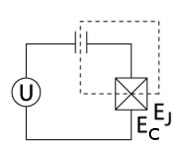
\includegraphics[width=.5\linewidth]{CPB-circuit.png}
  \caption{A diagram of the Cooper Pair Box. Note that $E_C$ and $E_J$
    are both parameters of the Josephson junction.}
  \label{cpb-circuit}
\end{figure}

One well-studied example of a quantum circuit is the Cooper Pair Box
(CPB)\cite{Nakamura,Vion}, see Fig.~\ref{cpb-circuit}. We used
the basic CPB as an initial test of our modeling techniques, and we
use it here as an introduction to the inductively-shunted Cooper pair
box (CPBL). The CPB is a superconducting circuit with three
components: a voltage source, a gate capacitor, and a Josephson
junction.

\begin{figure}
  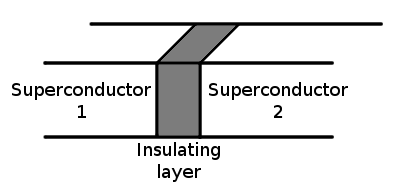
\includegraphics[width=.66\linewidth]{junction.png}
  \caption{ A sketch of a Josephson junction }
  \label{junction}
\end{figure}

The Josephson junction (Fig.~\ref{junction}) is a circuit element
consisting of two superconducting leads joined across a thin
insulating boundary. In our devices, Josephson junctions are
constructed by depositing a layer of aluminum, allowing a thin oxide
layer to form on the surface of that layer, and finally depositing a
second layer of aluminum on top. The oxide acts as an insulator, and
at sufficiently low temperatures the aluminum leads become
superconducting. A Josephson junction acts like a capacitor across its
insulating layer, but it also allows Cooper pairs of electrons to
tunnel through. We can treat the Josephson junction as a capacitor and
a tunneling junction in parallel, and we denote the energy scales
corresponding to these components as $E_C$ and $E_J$, respectively.

The Josephson tunnel junction, together with the gate capacitor,
creates a superconducting island in the CPB, indicated by the dotted
line in Fig.~\ref{cpb-circuit}. This lets us treat the CPB in its
``charge basis,'' where each state denotes a number of Cooper pairs
added to or removed from the island. In the charge basis, the
Hamiltonian of the CPB is
\begin{multline}
\label{cpb-H}
  H_{\text{CPB}} = \sum_{n=-\infty}^{+\infty} \left(\frac{-E_J}{2}\left(
      \ket{n}\bra{n-1} + \ket{n-1}\bra{n} \right)\right. \\
  \left.\phantom{\frac{-E_J}{2}} + 4E_C(n-N_g)^2\ket{n}\bra{n}\right),
\end{multline}
where $n$ represents the number of tunneled Cooper pairs and $N_g$ is
the offset charge across the capacitor, which is set by the gate
voltage according to $N_g=\frac{C_gV_g}{2e}$.

In order to calculate the energy spectrum of the CPB as a function of
the offset charge, we will need to express $H_{\text{CPB}}$ as a
matrix in the charge basis. Note that $H_{\text{CPB}}$ will be an
infinite matrix not just downward and rightward but, because $n$ and
$m$ can take all integer values, leftward and upward as well. Each
matrix element ${H_{\text{CPB}}}_{nm}$ is equal to the inner product
$\innerp{n}{H_{\text{CPB}}}{m}$, so specifying those inner products
specifies the matrix itself. Eqn.~\eqref{cpb-H} gives us:
\begin{equation}
  \innerp{n}{H_{\text{CPB}}}{m} = 
  \begin{cases}
    4E_C(n-N_g)^2 & \text{if $n=m$} \\
    \frac{-E_J}{2} & \text{if $|n-m|=1$}\\
    0 & \text{otherwise}
  \end{cases}
\end{equation}

Truncating this tridiagonal matrix allows us to approximate its
eigenvalues numerically. Up to an overall scale, the eigenvalues
depend only on the ratio between $E_J$ and $E_C$, and we can plot the
energy spectra relative to $N_g$ for several values of this ratio in
Figs. \ref{cpb-1}, \ref{cpb-10}, and \ref{cpb-30}. Units on the
y-axis are in gigahertz. We can see that for values where $E_C$ is
dominant (Fig.~\ref{cpb-1}) the spectrum looks like a series of
parabolas, which results from the quadratic term on the diagonal of
$H_{\text{CPB}}$. For larger values the spectral lines smooth out and
move apart, approaching a constant spacing.

\begin{figure}
  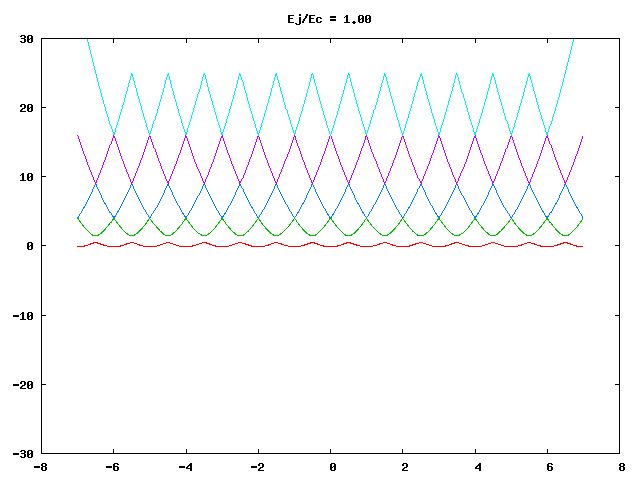
\includegraphics[width=\linewidth]{CPB-1.png}
  \caption{Energy spectrum vs. $N_g$ for the CPB with
    $\frac{E_J}{E_c}=1$}
  \label{cpb-1}
\end{figure}
\begin{figure}
  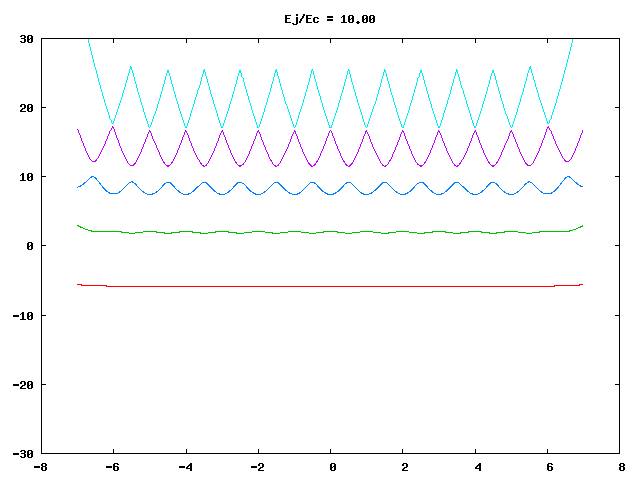
\includegraphics[width=\linewidth]{CPB-10.png}
  \caption{Energy spectrum vs. $N_g$ for the CPB with
    $\frac{E_J}{E_c}=10$}
  \label{cpb-10}
\end{figure}
\begin{figure}
  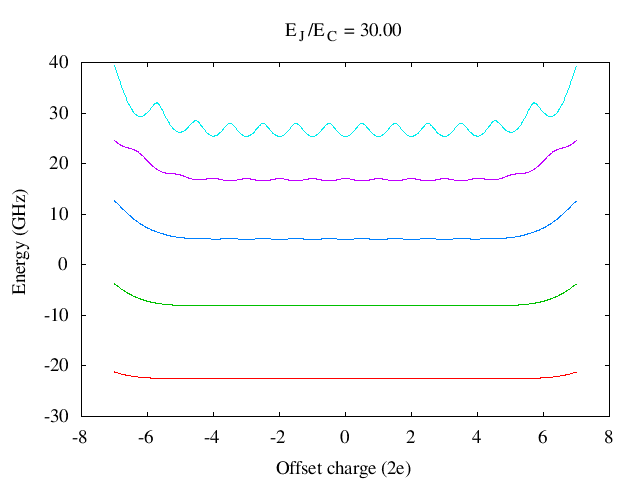
\includegraphics[width=\linewidth]{CPB-30.png}
  \caption{Energy spectrum vs. $N_g$ for the CPB with
    $\frac{E_J}{E_c}=30$. Note that the deviations from periodicity on
    the left and right ends of each line are artifacts of the
    approximation process, not of the theory itself. Extending the
    matrix cutoff pushes these deviations farther out in $N_g$.}
  \label{cpb-30}
\end{figure}

\section{Challenges with the CPB}
As with all quantum circuits, one of the primary goals is to obtain a
device with long decoherence times. In the case of the CPB, one of the
primary causes of decoherence is the charge noise---slow, randomly
oscillating charges in the environment that introduce noise into the
offset charge, $N_g$.

Several strategies exist for mitigating the effects of charge noise in
the CPB. One approach is to operate the device near local
extrema---the so-called ``sweet spots''---of the energy
spectrum \cite{Vion}. We can see in Fig.~\ref{cpb-1} that at certain
values of $N_g$ all of the spectral lines of the CPB reach local
maxima or minima. When the CPB is operated at these points, the first
order effects of charge noise drop out.

Another approach is to operate the CPB in the ``transmon'' region
where $E_J\gg E_C$ \cite{Koch}. We can see in Fig.~\ref{cpb-30} that the
spectral lines become very flat, reducing the effects of charge noise
even further. One of the disadvantages of working in the transmon
region is that, as we mentioned earlier, the spacing between spectral
lines becomes nearly uniform. Because a qubit generally needs to be
restricted to two energy states, this lack of anharmonicity can be a
substantial problem.

A third option---the option that we explore here---is to add an
inductive shunt to the CPB (Fig.~\ref{CPBL-circuit}). The energy
spectrum of the CPBL is entirely distinct from that of the CPB and
worthy of study in its own right, but it is also much less sensitive
to charge noise. This results from the fact that at low
frequencies---that is, at the frequencies of substantial charge
noise---the inductor acts like a closed circuit and shunts those
signals, while at high frequencies---like those of our input
voltages---the inductor approximates an open circuit, and the CPBL
behaves similarly to the CPB.

\section{Modeling the Inductively Shunted Cooper Pair Box}

\begin{figure}
  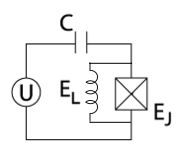
\includegraphics[width=.5\linewidth]{CPBL-circuit.png}
  \caption{ A diagram of the inductively shunted Cooper pair box
    (CPBL). The circuit now has three parameters, $E_C$ and $E_J$
    associated with the Josephson junction, and $E_L$ associated with
    the inductor. An external magnetic field creates a tunable
    magnetic flux, $\Phi$, through the superconducting loop.}
  \label{CPBL-circuit}
\end{figure}

Adding the inductor requires that we make several changes to our
equations. First, since no superconducting island exists in the CPBL,
the charge basis is no longer discrete. We will instead use another
basis from the CPB called the phase basis. The phase term arises from
the Josephson equations (see \cite{Feynman}). Expressed in the phase
basis, the Hamiltonian of the CPB takes the form
\begin{equation}
  H_{\text{CPB}} = -4E_C\frac{d^2}{d\varphi^2}-E_J\cos{\varphi}.
\end{equation}

Another consequence of the missing island is that no offset charge can
exist on the CPBL, and so we will instead plot the energy spectrum
with respect to $\Phi$, the magnetic flux through our inductor. The
$\Phi$ parameter comes into the picture when we add the term for our
inductor to $H_{\text{CPB}}$, producing the Hamiltonian
\begin{equation}
  H = -4E_C\frac{d^2}{d\varphi^2}-E_J\cos{\varphi}+\frac{1}{2}
  E_L\left(\varphi-\frac{2\pi\Phi}{\Phi_0} \right)^2,
\end{equation}
where $\Phi_0$ is the magnetic flux quantum, $\Phi_0 = h/2e$. This
equation also introduces a third design parameter for the CPBL, the
inductive energy, $E_L$. In order to analyze this equation, we will
immediately adopt a change of variables, $\varphi \rightarrow (\varphi
+ \frac{2\pi\Phi}{\Phi_0})$.
\begin{equation}
  \label{H}
  H = -4E_C\frac{d^2}{d\varphi^2}-E_J\cos\left(\varphi+
    \frac{2\pi\Phi}{\Phi_0}\right)+
  \frac{1}{2} E_L\varphi^2.
\end{equation}
After the change we can see that, apart from the cosine term in the
middle, $H$ takes the form of a simple harmonic oscillator (SHO). It
will therefore be convenient to express $H$ in the harmonic oscillator
basis over $\varphi$. Note that this is again a discrete basis, though
unlike the CPB, its matrix form extends infinitely only in the two
conventional directions. To facilitate calculations in this basis, we
separate $H$ into two pieces:
\begin{align}
  H & = H_0 + V\\
  H_0 & = -4E_C\frac{d^2}{d\varphi^2} +
  \frac{1}{2} E_L\varphi^2 \\
  V & = -E_J\cos\left(\varphi + \frac{2\pi\Phi}{\Phi_0}\right).
\end{align}
Simply substituting the coefficients in $H_0$ into the SHO equations,
with $\ket{n}$ now referring to SHO basis states over $\varphi$, gives
us that
\begin{equation}
  \innerp{n}{H_0}{m} = 
  \begin{cases}
    \sqrt{8E_LE_C}\left(n+\frac{1}{2}\right) & \text{if $n=m$} \\
    0 & \text{otherwise.}
  \end{cases}
  \label{inner-H0}
\end{equation}
The inner product with $V$, on the other hand, requires a fairly
complicated integral. The result is
\begin{equation}
  \innerp{n}{V}{m} = \left\{\begin{array}{l}
      -E_J(-2)^{-m'}\cos\left(\frac{2\pi\Phi}{\Phi_0}\right)\varphi_0^{2m'}\\
      \quad{}\times \sqrt{\frac{n'!}{(n'+2m')!}}
      \exp\left(\frac{-\varphi_0^2}{4}\right)\\
      \quad{}\times L_{n'}^{2m'}\left(\frac{\varphi_0^2}{2}\right)
      \phantom{{}^{{}+1}}\qquad \text{if $n \equiv m \pmod{2}$}\\
      -E_J(-2)^{-m'}\frac{1}{\sqrt{2}}\sin
      \left(\frac{2\pi\Phi}{\Phi_0}\right)\varphi_0^{2m'+1}\\
      \quad{}\times \sqrt{\frac{n'!}{(n'+2m'+1)!}}
      \exp\left(\frac{-\varphi_0^2}{4}\right)\\
      \quad{}\times L_{n'}^{2m'+1}\left(\frac{\varphi_0^2}{2}\right)
      \qquad\text{if $n \not\equiv m \pmod{2}$},
\end{array}\right.
\label{inner-V}
\end{equation}
where
\begin{align}
  n'& =\min(n,m)\\
  m'&=\left\lfloor\frac{|n-m|}{2}\right\rfloor \\
  \varphi_0 &=\sqrt[4]{\frac{8E_C}{E_L}},
\end{align}
and $L_n^\alpha$ is the generalized Laguerre polynomial.

Eqn.~\eqref{inner-V} is a ghastly expression but straightforward to
compute, so it and Eqn.~\eqref{inner-H0} specify $H$ entirely. As we
did with the CPB, we can now truncate this Hamiltonian and approximate
its eigenvalues numerically. Fig.~\ref{cpbl-theory} shows the spectrum
calculated as a difference from the ground state and plotted with
respect to magnetic flux, using a set of parameter values close to
those that our lab has tested experimentally.

\begin{figure} 
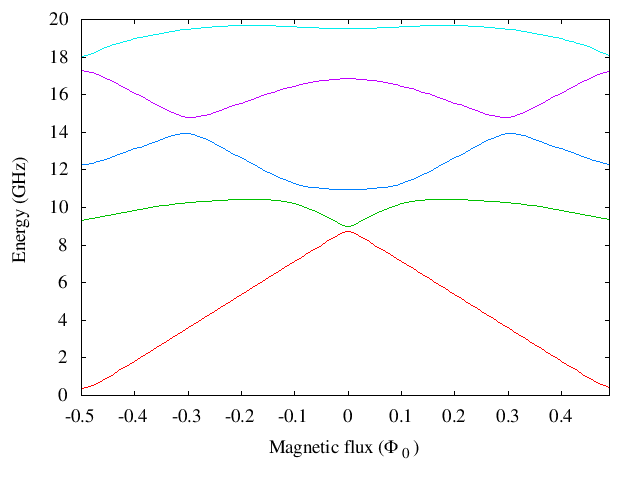
\includegraphics[width=\linewidth]{CPBL-theory.png}
\caption{ Energy spectrum (difference from the ground state) for the
  CPBL plotted against magnetic flux. $E_C=2.5$, $E_J=8.8$, and
  $E_L=0.5$. The y-axis and parameter values are given in gigahertz,
  and the x-axis is given in multiples of the flux quantum, $\Phi_0$,
  over one full period.}
\label{cpbl-theory}
\end{figure}

\section{Experimental Data}
\begin{figure}
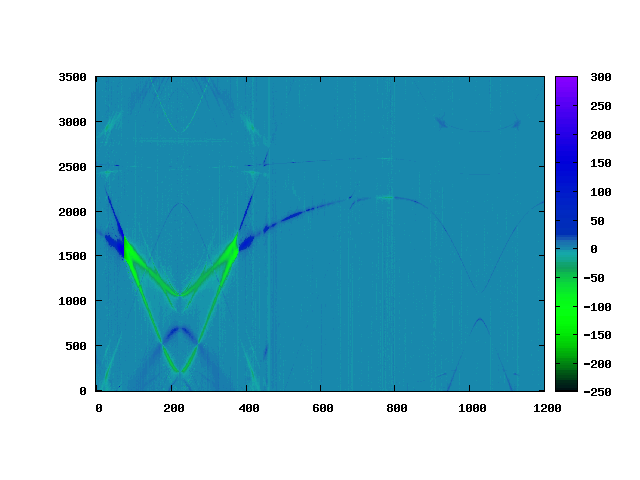
\includegraphics[width=\linewidth]{CPBL-color.png}
\caption{ Raw data from Vladimir Manucharyan. For scale, the avoided
  crossing on the bottom right of the image corresponds to the avoided
  crossing in the center of Fig.~\ref{cpbl-theory}. }
\label{raw}
\end{figure}

\begin{figure}
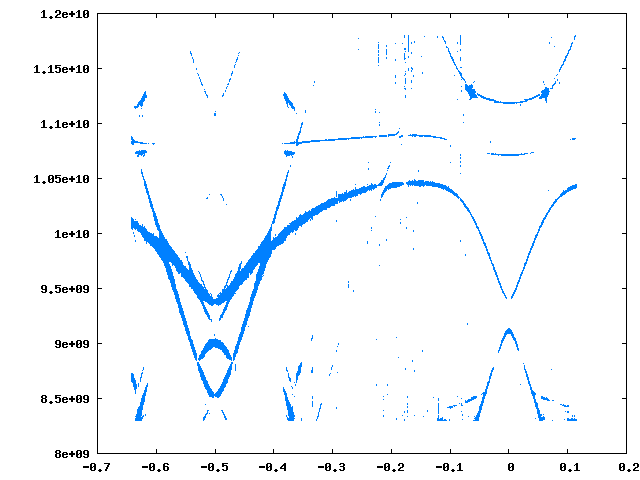
\includegraphics[width=\linewidth]{CPBL-data.png}
\caption{ Curves derived from the data in Fig.~\ref{raw} }
\label{filter}
\end{figure}

Vladimir Manucharyan has been measuring the energy spectra of the
first CPBL device ever produced, and one of the goals of this project
is to fit our theoretical spectra against his data. Energy curves were
originally drawn from those data by hand, but a simple threshold
filter can automate that process. Raw data (Fig.~\ref{raw}) can be
filtered into sets of points suitable for fitting
(Fig.~\ref{filter}).

There are many ways to define a ``badness of fit'' for theoretical
curves against these data. In our case, the simplest and most
effective method is, for each point in the data set, to find the
vertically nearest curve in the theoretical set, take the difference
between it and the data point, and add together the squares of these
differences. That is, for a given fit the badness, $B$, is defined as
\begin{equation}
\label{badness}
B = \sum_{p \in \text{data}} (t(p)-p)^2,
\end{equation}
where $t(p)$ is the closest point in the theoretical data set with the
same flux. We can then use generic multi-parameter minimization
routines to find the best fitting values of $E_C$, $E_J$, and
$E_L$ \cite{Byrd,Zhu}. The results of this approach are displayed
in Figs.~\ref{pre-fit} and \ref{post-fit}.

\begin{figure}
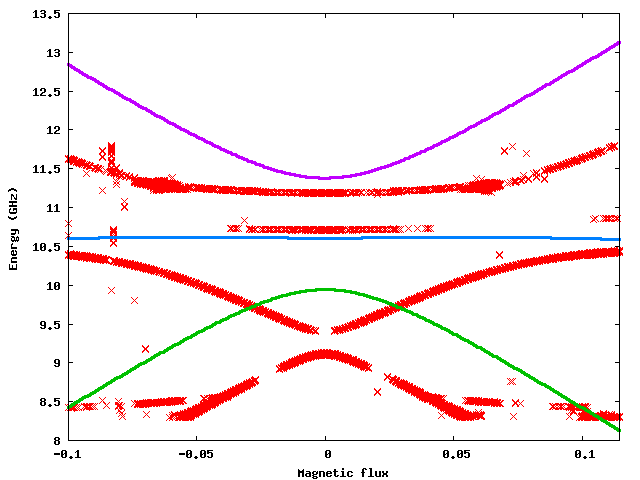
\includegraphics[width=\linewidth]{CPBL-prefit.png}
\caption{ An initial guess for parameter values plotted against
  experimental data from a portion of the set depicted in
  Fig.~\ref{raw}. This initial guess is clearly very poor, even
  though none of the parameters is off by more than 20\%.}
\label{pre-fit}
\end{figure}

\begin{figure}
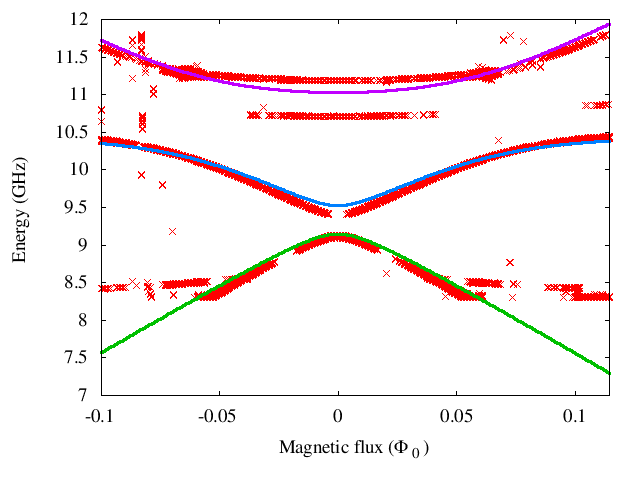
\includegraphics[width=\linewidth]{CPBL-postfit.png}
\caption{ The same data set from Fig.~\ref{pre-fit} after our
  optimization routines have adjusted the parameter values from the
  initial guess.}
\label{post-fit}
\end{figure}

The only additional input to the fit depicted in Fig.~\ref{post-fit}
is the initial parameter guess and the identification of the zero-flux
point on the x-axis. Note that the lines jutting out to the left and
right of the bottom peak in that figure represent a two-photon
transition, and the fit could be improved by including those
transitions. The line appearing clearly between the upper two spectral
lines in that figure is not one of these transitions but rather a
resonance from our experimental setup outside the CPBL itself, and it
causes the nearby lines to deviate slightly from the theory. Cleaning
out these extraneous points would improve the fit as well, though it
would be difficult to automate.

\section{Speeding it Up}

Simulation is one of the few areas left in programming where
computational speed remains a limiting factor. Mathematica models of
the CPBL built by Jens Koch already existed when we began this
project, and we used them to verify our results. They were fast enough
to generate the plots shown here but not fast enough to run that
computation over and over again to perform a fit. We used several
different optimizations to achieve the speeds necessary to perform
these fits.

The process of fitting a data set requires repeatedly calculating
energy spectra for different values of $E_C$, $E_J$, and
$E_L$. Calculating those spectra means repeatedly solving for the
eigenenergies of $H$ across a range of values of $\Phi$
values. Naturally, lots of work is duplicated when these calculations
are all performed in isolation. As it turns out, the most expensive
operation in our case is calculating the series expansions of the
generalized Laguerre polynomials to construct the $H$ matrix. Since
Laguerre polynomials obey a recursive relation, some time can be saved
by solving for all of them at once, rather than separately for each
element of $H$. However, a far more important realization is that,
while the term $L_n^\alpha(\varphi_0^2/2)$ depends on the circuit
parameters via $\varphi_0$, the coefficients in the series expansion
of $L_n^\alpha$ are independent of both $\Phi$ and the circuit
parameters. Thus all of those expansions only need to be calculated
once for an entire fitting procedure.

A similar speedup results from the fact that in all of
Eqns.~\eqref{inner-H0} and \eqref{inner-V}, only two terms in
Eqn.~\eqref{inner-V} depend on the value of $\Phi$. Thus the majority of
work needed to assemble $H$ can be done once for each trial of the
parameters $E_C$, $E_J$, and $E_L$, rather than for every value of
$\Phi$ plotted within that trial. That leaves only one trigonometric
term (either $\cos\left(2\pi\Phi/\Phi_0\right)$ or
($\sin\left(2\pi\Phi/\Phi_0\right)$) to be calculated and the
diagonalization operation to be performed for each value of
$\Phi$. These optimizations altogether speed up a fitting operation by
almost twenty times.

We achieved a second major speedup by taking advantage of the
capabilities of modern optimization algorithms \cite{Byrd,Zhu}.
Many of these algorithms calculate local partial derivatives in order
to improve their search for minima. Without assistance, these routines
can approximate local derivatives by evaluating several points in
close proximity, but it is also possible to supply these routines with
local derivative information we calculate ourselves. Rather than
having our routines evaluate the badness of a fit numerous times in a
small region around each set of trial parameters, we can calculate the
partial derivatives of the badness of fit in parallel with the fit
itself. As one might expect, calculating the derivatives this way
avoids lots of duplicated effort.

Recalling our definition of ``badness of fit'' in Eqn.~\eqref{badness},
the partial derivative for a given parameter $E_*$ is
\begin{equation}
  \label{partials}
  \frac{\partial B}{\partial E_{*}} =
  \sum_{p \in \text{data}}2(t(p)-p)\frac{\partial t}{\partial E_*}.
\end{equation}
The values of $t(p)$ are just differences among eigenvalues of $H$, so we
need to calculate the derivatives of those eigenvalues. Just how to do
that is not immediately obvious, but beginning with Schr\"odinger's
equation, we can develop a very convenient intermediate result.
\begin{equation}
  H\ket{\psi} = E\ket{\psi}
\end{equation}
Take the partial derivative of both sides.
\begin{equation}
  \frac{\partial}{\partial E_*} (H\ket{\psi}) =
  \frac{\partial}{\partial E_*} (E\ket{\psi})
\end{equation}
Expand via the product rule.
\begin{equation}
  \frac{\partial H}{\partial E_*}\ket{\psi} +
  H\frac{\partial}{\partial E_*}\ket{\psi} =
  \frac{\partial E}{\partial E_*}\ket{\psi} +
  E\frac{\partial}{\partial E_*}\ket{\psi}
\end{equation}
Multiply both sides by $\bra{\psi}$.
\begin{multline}
  \innerp{\psi}{\frac{\partial H}{\partial E_*}}{\psi} +
  \innerp{\psi}{H\frac{\partial}{\partial E_*}}{\psi} =\\
  \innerp{\psi}{\frac{\partial E}{\partial E_*}}{\psi}+
  \innerp{\psi}{E\frac{\partial}{\partial E_*}}{\psi}
\end{multline}
The $H$ in the second term comes out as a factor of $E$, and the third
term simplifies.
\begin{equation}
  \innerp{\psi}{\frac{\partial H}{\partial E_*}}{\psi} +
  E\innerp{\psi}{\frac{\partial}{\partial E_*}}{\psi} =
  \frac{\partial E}{\partial E_*} +
  E\innerp{\psi}{\frac{\partial}{\partial E_*}}{\psi}
\end{equation}
Finally, the two common terms cancel.
\begin{equation}
  \frac{\partial E}{\partial E_*} =
  \innerp{\psi}{\frac{\partial H}{\partial E_*}}{\psi}.
  \label{convenient}
\end{equation}
Eqn.~\eqref{convenient} leaves us with a very convenient formula for
calculating the partial derivatives of the eigenenergies of $H$.

Now, going back to Eqn.~\eqref{H}, we see that
\begin{align}
  \label{dC}
  \frac{\partial H}{\partial E_C} &= -4\frac{\partial}{\partial
    \varphi^2}\\
  \label{dJ}
  \frac{\partial H}{\partial E_J} &= \cos(\varphi +
  \frac{2\pi\Phi}{\Phi_0})\\
  \label{dL}
  \frac{\partial H}{\partial E_L} &= \frac{1}{2}\varphi^2.
\end{align}
Our eigenvalue routines can give us the eigenvectors $\ket{\psi}$
associated with each eigenvalue $E$ with little additional effort. In
the case of $\partial H/\partial E_J$, we have already calculated the
matrix form of Eqn.~\eqref{dJ}, namely the matrix $V$ without the extra
factor of $-E_J$, and taking the inner product of that matrix with
$\ket{\psi}$ gives us $\frac{\partial E}{\partial E_J}$.

In order to deal with Eqns.~\eqref{dC} and \eqref{dL}, we return to the
machinery of the SHO and recognize that
\begin{align}
  -4\frac{\partial}{\partial \varphi^2} &= -\sqrt{\frac{E_L}{2E_C}}
  (a-a^\dagger)^2\\
  \intertext{and}
  \frac{1}{2}\varphi^2 &= \sqrt{\frac{E_C}{2E_L}} (a+a^\dagger)^2.
\end{align}
We could express these operators in matrix form, but it is simpler and
faster to just apply the raising and lowering operators explicitly to
each eigenvector and dot the result with the original eigenvector.

Finally, we just sum up the partial derivatives using
Eqn.~\eqref{partials} just as we sum up the result with
Eqn.~\eqref{badness}. Calculating the derivatives ourselves, rather than
approximating them with extra function calls, nets us another speedup
of nearly a factor of four.

\section{Conclusion}
All the code for our project was written in Python, making extensive
use of the SciPy libraries. While Python is an excellent language for
fast prototyping, Python programs have a reputation for running
slowly, and at the beginning of our project it was unclear whether we
could realize substantial gains in efficiency without ultimately
switching to a faster platform. The fact that we achieved efficiency
gains of two orders of magnitude over our initial Python models
demonstrates that there was significant room for improvement both in
the algorithmics and in the mathematics of the CPBL model. At this
point, our code can fit a complete data set in one to two minutes, and
thinning out the data can bring that time down to about fifteen
seconds without significantly affecting the accuracy of the fit. We
hope that our code will help Vladimir Manucharyan and others as they
continue to explore the CPBL, and that the techniques we developed
will prove useful for implementing future models of the CPBL and other
systems.

\section{Acknowledgements}
Thanks to Steven Girvin, Luigi Frunzio, and Lev Bishop for discussions
about this project, to Vladimir Manucharyan, Rob Schoelkopf, and
Michel Devoret for the data we analyzed in this paper, and especially
to Jens Koch for his patient guidance.

\begin{thebibliography}{9}
\bibitem{Shor} P. W. Shor. ``Polynomial-Time Algorithms for Prime
  Factorization and Discrete Logarithms on a Quantum Computer.''
  \textit{SIAM Review}, Vol. 41, No. 2, pp. 303-332 (June 1999).

\bibitem{Grover} L. K. Grover. ``A fast quantum mechanical algorithm
  for database search.'' \textit{Proceedings of the twenty-eighth
    annual ACM symposium on theory of computing}, pp. 212-219 (1996).

\bibitem{Vandersypen} L. Vandersypen et al. ``Experimental realization
  of Shor's quantum factoring algorithm using nuclear magnetic
  resonance.'' \textit{Nature} 414, pp. 883-887 (20 December 2001).

\bibitem{Blais} A. Blais. ``Quantum information processing with
  circuit quantum electrodynamics.'' arXiv:cond-mat/0402216v1 (7
  February 2004).

\bibitem{Wallraff} A. Wallraff et al. ``Strong coupling of a single
  photon to a superconducting qubit using circuit quantum
  electrodynamics.'' \textit{Nature} 431, pp. 162-167 (9 September
  2004).

\bibitem{Nakamura} Y. Nakamura et al. ``Coherent control of
  macroscopic quantum states in a single-Cooper-pair box.''
  \textit{Nature} 398, pp. 786-788 (29 April 1999).

\bibitem{Vion} D. Vion et al. ``Manipulating the Quantum State of an
  Electrical Circuit.'' \textit{Science}, Vol. 3, No. 5569,
  pp. 886-889 (3 May 2002).
  
\bibitem{Koch} J. Koch et al. ``Charge insensitive qubit design
  derived from the Cooper pair box.'' arXiv:cond-mat/0703002v2 (28
  February 2007).

\bibitem{Feynman} R. P. Feynman, R. B. Leighton, and
  M. Sands. \textit{The Feynman Lectures on Physics}. Addison-Wesley
  Publishing Company. Vol. 3, Ch. 21-9 (1963).

\bibitem{Byrd} R. H. Byrd, P. Lu, and J. Nocedal. ``A Limited Memory
  Algorithm for Bound Constrained Optimization.'' \textit{SIAM Journal
    on Scientific and Statistical Computing} 16, 5,
  pp. 1190-1208 (1995).
  
\bibitem{Zhu} C. Zhu, R. H. Byrd, and J. Nocedal. ``L-BFGS-B, FORTRAN
  routines for large scale bound constrained optimization.''
  \textit{ACM Transactions on Mathematical Software} Vol 23, Num. 4,
  pp. 550 - 560 (1997).

\end{thebibliography}

\end{document}
